\section{Photon Detection System Overview}
\label{sec:fdsp-pd-ov}
%\metainfo{(Length: TDR=10 pages, TP=3 pages)}

%\fixme{Check citations are correct after build on the git hub (bibtex not working correctly on remote machine.}

%%%%%%%%%%%%%%%%%%%%%%%%%%%%%%%%%
\subsection{Introduction}
\label{sec:fdsp-pd-intro}


The photon detection (PD) system is an essential subsystem of the DUNE Single-Phase Far Detector (SPFD). The detection of the prompt scintillation light signal, emitted in coincidence with an ionizing event inside the active volume, allows the determination of the time of occurrence of an event of interest with much higher precision than charge collected from ionization in the TPC. This capability is most critical for the primary DUNE science objectives that are uncorrelated with the timing signal from the neutrino source at Fermilab, such as proton decay and neutrinos from a supernova burst, and for the ancillary science program including measurements of neutrino oscillation phenomena using atmospheric neutrinos.

Timing information from the PD and TPC systems allows determination of the drift time of the ionizing particles. Knowledge of the drift time provides localization of the event inside the active volume and provides the ability to correct the measured charge for effects that depend on the drift path length, purity of LAr, or for specific locations in the detector if there are non-uniformities.  This correction is important for the reconstruction of the energy deposited by the ionizing event. In addition to allowing optimum track reconstruction, scintillation light measured by the system may also be used as a trigger and for improved calorimetric measurement in combination with charge measurement.

Table~\ref{tab:pds-sys-req} summarizes the high level system performance requirements for the PD system necessary to achieve the DUNE science objectives. The first row provides a requirement to ensure high efficiency and good energy resolution for proton decay and atmospheric neutrinos.  The second row targets core collapse supernova burst neutrinos, but specifies only a timing measurement for event localization (in conjunction with the TPC drift time measurement). 
However, a consensus has emerged in the collaboration that the current requirements do not fully exploit the potential  for LAr scintillation light to contribute to the energy reconstruction of events, in particular for lower energy events such as from supernova neutrinos (\num{10}-\SI{100}{MeV}). In response, the third row is a proposed requirement to measure the energy in scintillation light from supernova neutrino events near the peak of the spectrum ($\sim$\SI{10}{MeV}) with a precision similar to that of the ionization measurement. The combined measurement of ionization charge and scintillation light has been shown to improve the determination of the energy deposition of an event. 
Table~\ref{tab:pds-det-req} shows the corresponding photon detection light yield, timing and spatial separation requirements. To achieve a 10\%  calorimetric measurement with light requires approximately ten times higher light yield for the PD system than the original requirement. 

%The first requirement is for minimum light yield of at least \SI{0.1}{photoelectrons(pe)/MeV}\fixme{what is the origin of this requirement - docDB indicates 1 pe/MeV at the center of the TPC} for events that occur near the cathode, which is the farthest region from photon collectors that are embedded in the Anode Plane Assembly (APA) (Chapter~\ref{ch:fdsp-apa}). 
%The second requirement is that the photon system will provide the timing of events relative to TPC timing, $t_0$, with a 
%resolution better than \SI{1}{$\mu$sec}.  The capability to measure the $t_0$ of non-beam events with deposited 
%energy above \SI{200}{MeV} will allow observation of proton decay and atmospheric neutrinos with high 
%efficiency by enabling 3D spatial localization of candidate events by the TPC. 

%The design described in this chapter is motivated by meeting these requirements, however, a consensus has emerged in the collaboration that a revision of these requirements should be considered in order to better exploit the characteristics of LAr scintillation light, in particular for lower energy events such as neutrinos from core collapse supernovae (10-100~MeV).
% and to improve the performance of the detector for low energy events such as neutrinos from core collapse supernovae. 

To achieve these requirements, there is an ongoing intense R\&D program to investigate methods that maximize the photon detection efficiency of the PD system within the constraints of the Single-Phase TPC design .  All three of the Photon Collector options described in this chapter could meet the original performance requirements, albeit with different event efficiency, but one, the ARAPUCA, has highest potential to perform the low energy calorimetric measurements at the desired precision. It also has the highest efficiency for supernova events and provides higher spatial granularity for background rejection. 


%\fixme{Update with requirements from docDB 112}

%\begin{dunetable}
%[Key performance requirements for the PD system (Note: these are under review).]
%{cc}
%{tab:pds-req}
%{Highest-level PD performance requirements to achieve the detection efficiency of $90$\% for energy deposit of \SI{> 200}{MeV}\fixme{what is the origin of this requirement - docDB indicates 1 pe/MeV at the center of the TPC} } 
%Requirement  & Value \\ \toprowrule
%Light Yield  & \SI{0.1}{pe/MeV} for events near the cathode plane  \\ \colhline
%Timing Resolution & \SI{1}{$\mu$s}   \\ \colhline
%\end{dunetable}

% rjw Requirements extracted from the global science and FD engineering requirements documents docDB 112}

\begin{dunetable}
[PD System performance requirements to achieve the primary science objectives.]
{p{0.45\textwidth}p{0.45\textwidth}}
{tab:pds-sys-req}
{PD System performance requirements to achieve the primary science objectives (under review).} 
Requirement  	& Rationale \\ \toprowrule
The far detector photon system shall detect sufficient light from events depositing visible energy >\SI{200}{MeV} to efficiently measure the time and total intensity. 
			& This is the region for nucleon decay and atmospheric neutrinos. The time measurement is needed for event localization for optimal energy resolution and background rejection.			\\ \colhline
The far detector  photon system shall detect sufficient light from events depositing visible energy <\SI{200}{MeV} to provide a time measurement.  The efficiency of this measurement shall be adequate for supernova burst events. 
			& Enables low energy measurement of event localization for supernova burst events. The efficiency may vary significantly for visible energy in the range \SI{5}{MeV} to \SI{100}{MeV}. 		\\ \colhline
(Proposed) The far detector photon system shall detect sufficient light from events depositing visible energy of  \SI{10}{MeV} to provide an energy measurement with a resolution of 10\%. 
			& Enables energy measurement for supernova burst events with a precision similar to that from the TPC ionization measurement. \\ \colhline
The far detector photon system readout electronics shall record time and signal amplitude from the photosensors with sufficient precision and range to achieve the key physics parameters. 
			& The resolution and dynamic range needs to be adjusted so that a few  photoelectron signal can be detected with low noise.  The dynamic range needs to be sufficiently high to measure light from a muon traversing a TPC module.  \\ 
\end{dunetable}

\begin{dunetable}
[Preliminary photon detector performance requirements.]
{p{0.45\textwidth}p{0.45\textwidth}}
{tab:pds-det-req}
{Photon detector performance requirements (under review). } 
Parameter  					& Value \\ \toprowrule
(Current) Minimum detector response per MeV energy deposition (Light Yield).
  							& \SI{1}{pe/MeV} for events at the center of the TPC and no less than \SI{0.5}{pe/MeV}  at all points in the fiducial volume. \\ \colhline
(Proposed) Minimum detector response per MeV energy deposition (Light Yield).
  							& \SI{10}{pe/MeV} for events at the center of the TPC and no less than \SI{5}{pe/MeV}  at all points in the fiducial volume. \\ \colhline
Minimum requirements on energy deposition, spatial separation, and temporal separation from other events, for which the system must associate a unique event time ({\it flash matching}). 
							& \SI{10}{MeV}, \SI{1}{m}, \SI{1}{ms}  respectively. \\
\end{dunetable}


%%%%%%%%%%%%%%%%%%%%%%%%%%%%%%%%%%%%%
\subsection{Design Considerations}
\label{sec:fdsp-pd-des-consid}
%\todo{\color{blue} Content: Segreto/Warner/Mualem}

\emph{Scintillation Light:} Liquid argon (LAr) is known to be an abundant scintillator and emits about \SI{40}{photons/keV} when excited  by minimum ionizing particles\cite{Doke:1990rza},
%There are a number of others possible - see email from ES 4/11/18
in the absence of external electric fields. In the presence of electrics fields the yield is reduced due to recombination; for the nominal DUNE SP TPC field of \SI{500}{V/cm} the yield is approximately \SI{24}{photons/keV.}\cite{PhysRevB.20.3486}. 
% From ES:  "Dynamical behavior of free electrons in the recombination process in liquid argon, krypton, and xenon", S.Kubota, M.Hishida, M.Suzuki, J.Ruan(Gen), Phys. Rev. B20 (1979), 3486 and Ruan(Gen), Jian-zhi, 

As depicted in Figure~\ref{fig:scintAr}, the passage of ionizing radiation in LAr produces excitations and ionization of the argon atoms that ultimately results in the formation of the excited dimer Ar$^*_2$.  
Photon emission proceeds through the de-excitation of the lowest lying singlet and triplet excited states, $^{1}\Sigma$ and 
$^{3}\Sigma$ to the dissociative ground state. The de-excitation from the $^{1}\Sigma$ state is very fast and has a characteristic time of the order of 
$\tau_{fast}$ $\simeq$ \SI{6}{ns}. The de-excitation from the $^{3}\Sigma$, state is much slower with a characteristic time of $\tau_{slow}$ $\simeq$ \SI{1.3}{$\mu$sec}, since it is forbidden by the selection rules. 
In both decays, photons are emitted in a \SI{10}{nm} band centered around \SI{128}{nm}, which is in the Vacuum Ultra-Violet (VUV) region of the electromagnetic spectrum.
The relative intensity of the  fast and slow components is related to the ionization density of LAr and depends on the ionizing particle: \num{0.3} for electrons, \num{1.3} for alpha particles and \num{3} for neutrons\cite{PhysRevB.27.5279}.
% From ES 4/11/18: A. Hitachi et al., Effect of ionization density on the time dependence of luminescence from liquid Ar and Xe, Ph. Rev. B 27 (1983), 5279;
This phenomena is the basis for the  particle discrimination capabilities of LAr exploited by many experiments that have the capacity to separate the two components, for DUNE the greatest significance relates to a pending decision on treatment of light signals.
%\fixme{Are we proposing to do this (is it better than TPC dE/dx)? If not there is there a point to emphasizing it?}

\begin{dunefigure}[Schematic of scintillation light production in argon.]{fig:scintAr}
{Schematic of scintillation light production in argon.}
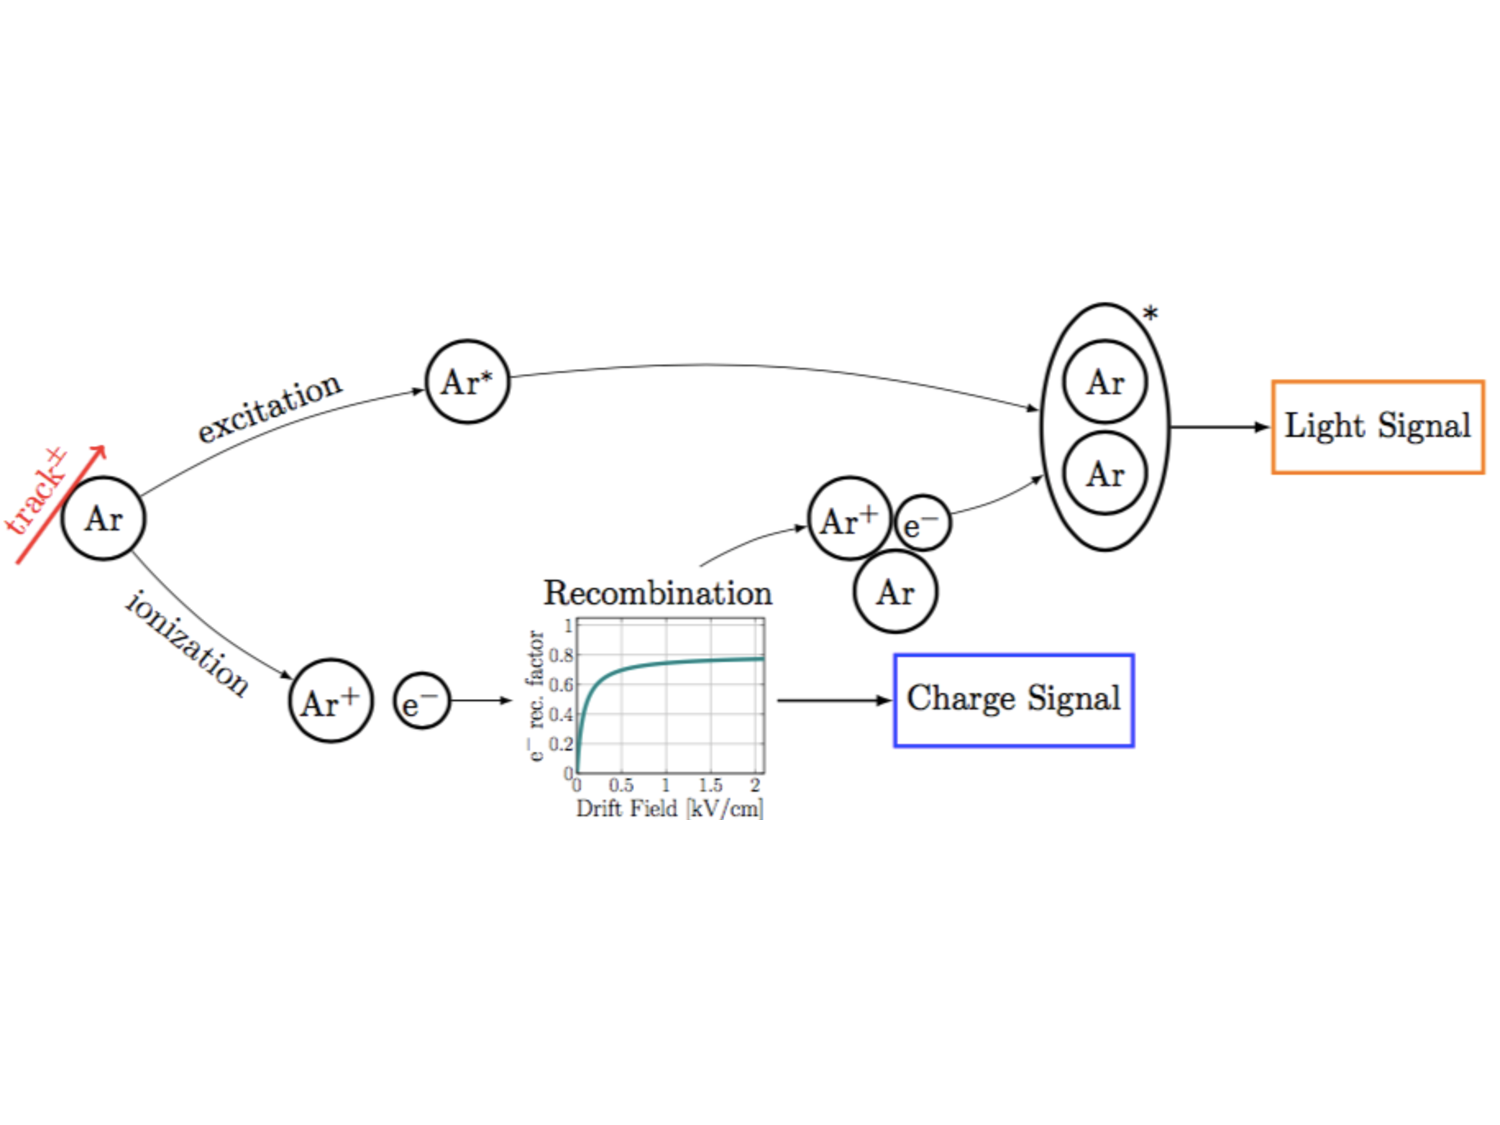
\includegraphics[width=0.8\columnwidth]{pds-scintAr-dppd_6_0.pdf}
\end{dunefigure}

In massive LAr TPCs, a cost-effective approach is to use photon collector systems that collect light from large areas and attempt channel it in an efficient way towards much smaller photosensors that produce an electrical signal.
This paradigm for the detection of LAr scintillation light depends on the use of chemical wavelength shifters since most currently available commercial (cryogenic) large area photosensors are not directly sensitive to VUV radiation, primarily due to the lack of transparency of fused silica and glass optical windows. 

\emph{\Ar39:}  The long-lived cosmogenic radioisotope \Ar39 has a natural abundance with an activity of approximately \SI{1}{Bq/kg} and
undergoes beta-decay with a mean beta energy of \SI{220}{keV} with an end-point of \SI{565}{keV}. In the \SI{10}{kt} far detector modules this leads to a rate of more than \SI{10}{MHz} of very short ($\sim$\SI{1}{mm}) tracks uniformly distributed throughout the detector module, each of which produces several thousand VUV scintillation photons. This continuous background impacts the DAQ, trigger and spatial granularity required of the PD system.
% rjw Wiki has ($1.01\pm0.08$) Bq/kg, but 1 is good enough for the purpose here.

\emph{Wavelength Shifter:} The most widely used wavelength shifter used in combination with LAr is Tetra-Phenyl Butadiene (TPB)\footnote{1,1,4,4-Tetraphenyl-1,3-butadiene, supplier: Sigma-Aldrich\textregistered.}, which absorbs VUV photons and re-emits them with a spectrum centered around \SI{420}{nm}, close to where most commercial photosensors have their maximum quantum efficiency for photoconversion. 
Though TPB has been studied quite extensively with great success, there are recent publications that warrant caution. For example, until recently the conversion efficiency of TPB in coating was taken to be high, approaching or even exceeding 100\% (possible by multi-photon emission), however a recent arXiv paper\cite{Benson:2017vbw} refutes this previous frequently referenced result. Using much of the same equipment but replacing a damaged reference photodiode, the authors (including an author of the previous paper) report a measurement for the quantum efficiency of 40\% for incident \SI{128}{nm} light. 
Another recent paper\cite{Asaadi:2018ixs} reports that some methods used to coat surfaces with TPB suffered loss of the TPB coating in LAr, whereas there is no measurable effect if the fluor is dissolved in a polymer matrix. These developments will be followed carefully and highlight the importance of the ongoing R\&D and prototype program.


%TPB conversion efficiency is known to be high, there is evidence that it approaches 100\% but reliable direct confirmation of this is not available in the literature\cite{Benson:2017vbw}. - april 2018
%Benson, V. Gehman et al. Retraction of earlier VG work - off by a factor of three due to bad reference photodiode! 
% Old paper VG with wrong results: Fluorescence Efficiency and Visible Re-emission Spectrum of Tetraphenyl Butadiene Films at Extreme Ultraviolet Wavelengths - Nucl.Instrum.Meth. A654 (2011) 116-121
%Tetraphenyl Butadiene Emanation and Bulk Fluorescence from Wavelength Shifting Coatings in Liquid Argon - 	arXiv:1804.00011 [physics.ins-det] April 2018

\emph{Physical Constraints:} The physical dimension of the PD system is constrained by the need to fit within the innermost wire planes of the Anode Plane Assembly (APA) and to be installed through slots in the APA mechanical frame after it is wound (see Section~\ref{sec:fdsp-apa-design}). 
Individual photon detector modules will be restricted to be within an envelope in the form of a long, thin box. At the time of preparation of this proposal the dimensions were \SI{14.6}{cm} $\times$ \SI{9.6}{cm} $\times$ \SI{212.7}{cm}, but it is anticipated that the size of the slot in the APA will be increased by about 25\% (the long dimension of the modules will remain the same). There will be ten PD modules per APA, for a total of \num{1500} modules.

% The bars are l(less than \SI{1}{cm} thick)

%%% rjw 
\subsubsection{Photon Collectors} 
\label{sssec:photoncollectors}

The core modular elements of the PD system are the large area {\it photon collectors} that convert incident \SI{128}{nm} scintillation photons into photons in the visible range (>\SI{400}{nm}), which in turn are converted to an electrical signal by compact silicon photomultipliers (SiPM). 
As detailed in Section \ref{sec:fdsp-pd-design}, since the size and cost of currently available SiPMs are not well-matched to meeting the performance requirements in the large volume  SPFD, the photon collector design aims to maximize the active VUV-sensitive area of the photon detection system module while minimizing the necessary photocathode (SiPM) coverage. 
In the following we will distinguish between the terms photon {\it collection} efficiency and photon {\it detection} efficiency. Collection efficiency is the number of visible photons delivered to the SiPM(s) divided by the number of VUV photons incident on the PD module active area; this parameter is used to report results of calculations or simulations of predicted device performance independent of the SiPM used.  Detection efficiency is the number of detected photoelectrons (pe) from the SiPM(s) divided by the number of VUV photons incident on the PD module active area; this is generally the result of a direct measurement unless the detailed performance of the SiPM is known and divided out. The {\it effective area} of a PD module is another useful figure-of-merit that is defined to be the photon detection efficiency multiplied by the photon collecting area of a PD module. 

Three different designs of PD photon collector modules have been developed and are being considered by the Single-Phase Photon Detector (SPPD) Consortium. The baseline design, ARAPUCA\footnote{{\it Arapuca} is the name of a simple trap for catching birds originally used by the Guarani people of Brazil.}, is a relatively new concept that is scalable and has the potential for the best performance of the three designs by a significant factor. It is functionally a light trap that captures wavelength-shifted photons inside boxes with highly reflective internal surfaces where they are eventually detected by SiPMs.  There are also two alternative designs based on the use of wavelength-shifters and light guides coupled to SiPMs. Both have undergone more development than ARAPUCA but their performance meets the basic physics requirements with only a limited safety margin and are not easily scalable within the geometric constraints of the Single-Phase detector.
Figure~\ref{fig:3dtpc-pd} shows a 3-D model of the Single-Phase TPC with a zoom in to the anode plane where the three candidates photon collector technologies are visible for illustration - in the final detector there will be a single type.
%%%%%%%%%%

\begin{dunefigure}[3-D model of photon detectors in the APA.]{fig:3dtpc-pd}
{3-D model of photon detectors in the APA. The model on the left shows the full width of the TPC with the configuration APA-CPA-APA-CPA-APA. The figure on the right shows a zoom in to the top far side of the TPC where three candidates photon collector technologies are visible for illustration - in the final detector there will be a single type.}
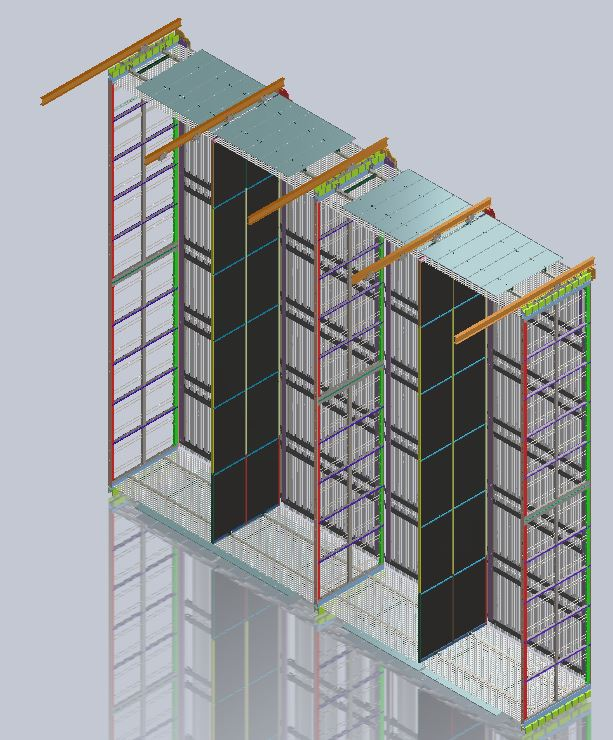
\includegraphics[height=6cm]{pds-dune-sp-tpc-3d.jpg}
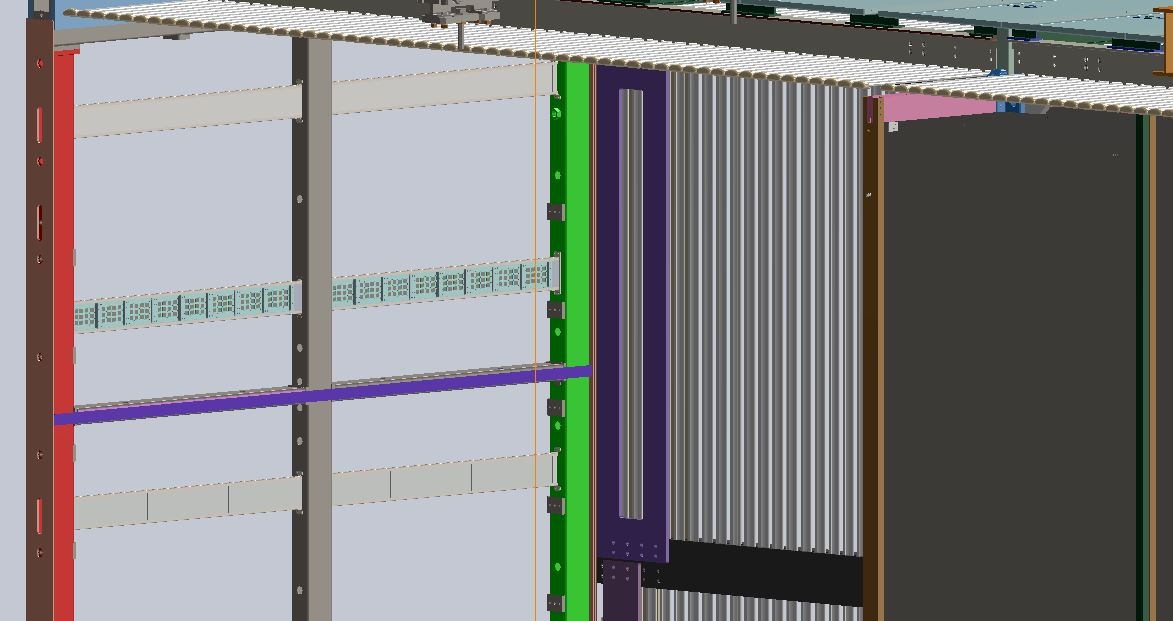
\includegraphics[height=6cm]{pds-dune-sp-tpc-3d-zoom.jpg}
\end{dunefigure}


{\it\bf ARAPUCA Option:} The first large-scale implementation of an ARAPUCA module in ProtoDUNE-SP is composed of an array of sixteen ARAPUCA cells each one acting as an individual detector element. This configuration allows for finer spatial segmentation along the detector bar than is the case for the light guide designs. 
The ProtoDUNE-SP ARAPUCA design collects light from one side of the box through an optical window formed  
by a dichroic filter deposited with a layer of pTP\footnote{p-TerPhenyl,  supplier: Sigma-Aldrich\textregistered.}
% https://www.sigmaaldrich.com/catalog/substance/pterphenyl230309294411.} 
wavelength shifter on the external surface that shifts the incident VUV light to a near-visible frequency able to pass through the filter plate to the interior of the box.  
In the ProtoDUNE-SP version of the device, the inner surface of the box opposite the window houses an array of SiPMs that cover a small fraction of the area of the window (2.8-5.6\%), surrounded by a foil of a highly reflective material coated with a second wavelength shifter, TPB. The TPB
converts the light passing through the filter to a wavelength that will be reflected by the filter. It has been shown in simulation and in prototypes that a large fraction of these trapped photons, reflecting from the filter and the lined walls of the box, will eventually fall on an SiPM and be detected.
The X-ARAPUCA described in Section~\ref{sssec:x-arapuca}, is a promising variant of the concept that uses a wavelength shifter-doped plate between two dichroic filter windows with SiPMs on the narrow sides of the cell; in addition to viewing scintillation light from both sides as needed for the central APA, it is expected to provide a higher light collection efficiency.

%ARAPUCAs that will be mounted in the central APA frame will need to collect light from both directions. In this case filter plates can be mounted on both sides of the box and the SiPMs moved to the walls.  Here, the TPB is coated directly onto the inner surface of the filter plates or is embedded in a plate between the windows in the case of X-ARAPUCA. 

The ARAPUCA concept is relatively recent -- it was first proposed in 2015 and accepted for installation in ProtoDUNE-SP in mid-2016. A series of tests in LAr have been performed with an evolving prototype design that resulted in detection efficiency measurements ranging from  \num{0.4}\% to \num{1.8}\%, demonstrating the potential for substantially higher performance than the light-guide designs. Monte Carlo simulations show that detection efficiencies at the level of several per cent could be reasonably reached with improvements to the basic design. 
While the results of the experimental tests are encouraging, a deeper understanding of the optical phenomena involving emission and scattering on wavelength-shifter coated surfaces is needed to optimize the design.

{\it\bf Light Guide Options:} The fundamental idea of this approach is to convert VUV scintillation light to visible wavelengths on (or near) the surface of an optical light guide, which then guides some fraction of the converted light by total internal reflection to SiPMs mounted on one or both ends of the guide.

Several approaches were investigated and narrowed down to the two most promising ones based a set of comparative measurements taken simultaneously in LAr~\cite{Whittington:2015rkr}. These two have been improved over several years and have reached a reasonable level of maturity and reliability.
The {\it dip-coated} light guides are pre-treated commercially-cut acrylic bars that are dip-coated with a solution of TPB, acrylic, and toluene. When the toluene evaporates it leaves a thin film of TPB embedded in the acrylic matrix on the surface of the bar.  In the {\it double-shift} light guides, the conversion and guiding processes of the photons are decoupled. The first conversion is in a {\it radiator plate}, which is an ultraviolet transmitting UVT-acrylic plate coated with pure TPB through a spraying process. It is positioned 
%\SI{1}{mm} 
just above a commercial WLS-doped bar that absorbs the blue light produced by TPB and re-emits it in the green; a fraction of this green light propagates down the bar. 

Both bar designs have demonstrated attenuation lengths for the  trapped light along the long dimension of the bar comparable to the length of the bars themselves, which ensures a reasonable uniformity along the beam direction. Preliminary measurements of both designs with readout at just one end indicate an photon detection efficiency range of  \num{0.1}\% to \num{0.25}\% averaged along the length of the bar. 
%\fixme{Numbers to be confirmed.} See response from Stu Mufson March 2018.
%Their absolute efficiency has been measured to be in a range between \num{0.1}\% and \num{0.2}\%.
%DWW 15mar18 start %%%%%%
%\fixme{Does IU report efficiency closer to .3 or .4 \%  for the double-dip --email sent to Stu \& Denver}
%DWW 15mar18 end %%%%%%
Up to a factor of four higher detection efficiency might be achieved with straightforward enhancements, such as:  SiPM at both ends of the bars; higher PDE SiPMs; and coating the long edges of the bars with reflective foils. 

\subsubsection{Wavelength Shifter-Coated Cathode Plane} 
Since the photon detection modules are installed only on the anode plane, light collection is not uniform over the entire active volume of the TPC. A possible solution to improve this is to install a reflective foil coated with wavelength shifter on the cathode.
This would increase the light yield of the detector and could enable calorimetric measurements based on light emitted by the ionizing particles. It may also be possible to remove the \Ar39 background through PD-supplied timing cuts, a background that may otherwise cause a huge counting rate for events near the anode plane. This option would require good visible light sensitivity for the photon collectors, which is not the case for current light collector options. The capability could be incorporated in a variety of ways but with an impact on the direct light measurement. This option has yet to be formally adopted by the PD Consortium but is under study through Monte Carlo simulations and the mechanical feasibility is being discussed with the HV Consortium.

\subsubsection{Silicon Photosensors} 
In each photon collector concept, the final stage of converting a visible wavelength photon into an electrical signal will be performed by a SiPM. The device must operate reliably for many years at LAr temperatures.
Our experience with a promising early candidate that failed in later batches, due to an unadvertised change in the fabrication process, has emphasized the importance of a multi-source approach where we are actively engaged with potential vendors to develop a device expressly for cryogenic operation. Currently, there are ongoing investigations of MPPCs (Multi-Pixel Photon Counter) produced by Hamamatsu (Japan) including a model specifically designed for cryogenic operation, and a device developed for operation in LAr by FBK (Fondazione Bruno Kessler, Italy) in collaboration with the DarkSide experiment.

\subsubsection{Readout Electronics} 
For prototype development and for ProtoDUNE-SP, a waveform digitizer has been developed that enables a thorough investigation of the photosensor signals, particularly as we investigate the impact of electrically ganging multiple SiPMs. The design of the readout electronics for the final system will be strongly influenced by the outcomes of Monte Carlo simulations that are in progress. Of particular interest is the extent to which pulse  shape capabilities are important to maximizing sensitivity to low energy neutrino interactions from supernovae. 
Initial Monte Carlo simulations suggest that it may not be necessary to fully digitize the SiPM waveforms in order to achieve the PD performance requirements.  Charge integration electronic readout systems, which offer the promise of significantly lower cost and smaller cabling harnesses, are under investigation and is expected to be the baseline solution.
A lower-cost waveform digitization based on lower sampling rate commercial electronics will be investigated as a potential backup option in case our evolving understanding of the requirements necessitates collecting waveform data from the SiPMs.

The size of currently available SiPMs is far smaller than the spatial granularity required for the experiment so the output of individual devices will be electrically summed (ganged) to reduce the electronics channel count. This will be achieved either by simply connecting together the output of multiple devices, passive ganging, or using active components, active ganging, if the signal is too degraded. Both approaches are under investigation. 

\subsubsection{R\&D Priorities} 
Since the light-guide designs are comparatively well-understood, the need for an improved understanding of the potential ARAPUCA performance drives the strategy for the R\&D program that will be carried out before the Technical Design Report (mid-2019). 
An intense effort is underway to demonstrate that an implementation of the ARAPUCA concept will increase the light yield of the detector by a factor of five to ten with respect to the light guides; resources (personnel and funding)  are being sought by the Consortium to achieve this.  Since the ARAPUCA approach demands a larger number of SiPMs than the light guides, a related high priority is demonstration of active ganging of a sufficient number of devices with adequate signal-to-noise properties.

It is anticipated that by the time of the TDR, the Consortium will present ARAPUCA as a baseline design for the photon collector with one alternative design for risk mitigation.  

%DWW 15mar18 end %%%%%%

\subsection{Development and Evaluation Plans}
%\todo{\color{blue} Content: Segreto}

The performance of the different photon collection options will be evaluated at several facilities available to the Consortium. 
Relative and absolute measurements will be performed at both room and cryogenic temperatures.

The most comprehensive set of data will come from the fully instrumented modules in the ProtoDUNE-SP experiment currently 
under construction at CERN, which will start operations in the last third of \num{2018}.
All  three photon collector designs are present in ProtoDUNE-SP: \num{29} 
double-shift guides, \num{29} dip-coated guides, and two ARAPUCA arrays. 
The TPC will provide precise reconstruction in 3D of the track of any ionizing event inside the active volume and matching  
the track with the associated light signal will enable an accurate comparison of the relative detection efficiencies of the different PD modules. 
In principle, absolute measurements are possible using Monte Carlo simulations, but currently some of the optical parameters that 
regulate VUV light propagation in LAr are poorly known,
%such as Rayleigh scattering length, 
which will limit the precision of the absolute  measurements. 
A plan will be developed to address this limitation.
%\todo{sounds like we need a plan to measure this somewhere...}

ProtoDUNE-SP will also provide a long-term test of full-scale PD modules for the first time so it may be possible to quantify any deterioration in their performance such as the loss of TPB from the coating noted previously. 
More broadly, aging effects in various detectors technologies, such as scintillator and photomultipliers tubes, are well-documented and knowledge of such effects is required at the design stage so that the photon detection performance will meet minimum requirements for the whole life of the experiment.

An R\&D program will be executed in parallel with the ProtoDUNE-SP operation since additional comparative measurements will be needed, particularly for the newer ARAPUCA concept, prior to establishing the baseline design for the Technical Design Report.
%DWW 15mar18 start %%%%%%
%The TallBo facility at Fermilab will be extremely important for this program. 
%It provides a \SI{450}{liter} capacity cryostat with \SI{56}{cm} inner diameter and up 
%to a \SI{183}{cm} liquid depth that accommodates  up to three different PD 
%modules with dimensions \todo{how different?} close to the real ones.
% I think we should cut this
%DWW 15mar18 end %%%%%% rjw edits
Several facilities are accessible to the Consortium that will allow testing of smaller scale prototypes of the modules (or sections of them). 
These include: the cryogenic facilities 
%ScENE set-up 
at Fermilab,  Colorado State University and Universidade Estadual de Campinas (UNICAMP); and facilities for precision optical measurements and cryogenic testing of photosensors at Fermilab, Indiana University, Northern Illinois University, University of Iowa, Syracuse University, UNICAMP, and Institute of Physics in Prague. 

%DWW 15mar18 start %%%%%%

A critical issue for large experiments are the interfaces between the sub-systems. PD modules and interfaces with the APA system and cold electronics will be conducted using cryogenic gaseous nitrogen in cold box studies at CERN, using a test stand developed for testing of ProtoDUNE-SP components prior to installation into the detector.  A full-scale ProtoDUNE-SP APA is currently being fabricated, and will be instrumented with cold electronics and photon detectors, allowing the interfaces to be carefully studied.

In addition, a small-scale TPC is planned for cold electronics testing at FNAL, and will be instrumented with as many as three 1/2-length PD modules to provide triggering information for the TPC and to continue interface studies with the APA and cold electronics.  It is envisioned that up to three test cycles will be performed prior to the TDR, allowing testing and continued development of the ARAPUCA concept.
%DWW 15mar18 end %%%%%%
%These facilities will be valuable for the single modules optimization process.

%Timeline appears in the last section.
%A decision on the light collector technology will be made in February 2019.

%\subsection{Scope}
%\label{sec:fdsp-pd-scope}
%\todo{\color{blue} Content: Segreto/Warner/Mualem}
%\fixme{The "Scope" section that was here (part of the original lead editors template) is rather "projecty" and just a list of the system components. It seems out of place - removed unless the editors insist to put it back!.}
% Removal agreed by the editors 4/11/18
%
%The scope of the photon detector (PD) system for the DUNE far detector 
%reference design includes design, procurement, fabrication, testing,
% delivery and installation of the following components:
%\begin{itemize}
%       \item light collection system;
%        \item photosensors (silicon photomultipliers);
%        \item readout electronics and cabling;
%        \item calibration system (tbd);
%        \item (TPB-coated foils for the cathode plane (if implemented));
%        \item related infrastructures.
%\end{itemize}